\subsection{Towards General Data Management Policies}
\label{sec:scope}

\begin{figure*}[t!]
    \centering
    \ssp
    \begin{subfigure}[t]{0.48\textwidth}
        \centering
        \tiny
        \centering
        \begin{minted}[xleftmargin=3em,linenos]{lua}
function when()
  if server[whoami]['cachesize'] > n then
    if server[whoami]['cachesize'] > 100K then
      WRstate(1)
    end
    if RDstate() == 1 then
      return true
    end
  end
  return false
end
        \end{minted}
        \caption{ParSplice cache management policy that absorbs the burstiness of the
        workload before switching to a constrained cache.  The
        performance/utilization for different  \(n\) is in
        Figure~\ref{fig:methodology-tradeoff}. \label{src:lru-dyn}}
    \end{subfigure}%
    ~ 
    \begin{subfigure}[t]{0.48\textwidth}
        \centering
        \tiny
        \begin{minted}[xleftmargin=3em,linenos]{lua}
local function when()
  if servers[whoami]["load"] > target then
    overloaded = RDstate() + 1
    WRstate(overloaded)
    if overloaded > 2 then
      return true
    end
  end
  else then WRstate(0) end
  return false
end
        \end{minted}
	\caption{CephFS file system metadata load balancer, designed in 2004
        in~\cite{weil:sc2004-dyn-metadata}, reimplemented in Lua
        in~\cite{sevilla:sc15-mantle}. This policy has many similarities to the
        ParSplice cache management policy.\label{src:lua-cephfs}}
    \end{subfigure}
    \dsp
    \caption{ParSplice's cache management policy has the same components as
    CephFS's load balancing policy.}
\end{figure*}

In the previous section, we used our data management language and the Mantle
policy engine to design effective cache management strategies for a new
application and storage system. In this section, we compare and contrast the
policies examined for file system metadata load balancing
in~\cite{sevilla:sc15-mantle} with the ones we designed and evaluated above for
cache management in ParSplice. 

\subsubsection{Using Load Balancing Policies for Cache Management}

%- memory utilization/heuristics
From a high-level the cache management policy we designed in
Figure~\ref{src:lru-dyn} trims the cache if the cache reaches a certain size
{\it and} if it has already absorbed the initial burstiness of the workload.
Much of this implementation was inspired by the CephFS metadata load
balancing policy in Figure~\ref{src:lua-cephfs}, which was presented
in~\cite{sevilla:sc15-mantle}. That policy migrates file system metadata if the
load is higher than the average load in the cluster {\it and} the current
server has been overloaded for more than two iterations. The two policies have
the following in common:

\textbf{Condition for ``Overloaded"} (Fig.~\ref{src:lru-dyn}: Line 2;
Fig.~\ref{src:lua-cephfs}: Line 2) - these lines detect whether the node is
overloaded using the load calculated in the load callback (not shown). While
the calculations and thresholds are different, the way the loads are used is
exactly the same; the ParSplice policy flags the node as overloaded if the
cache reaches a certain size while the CephFS policy compares the load to other
nodes in the system.

\textbf{State Persisted Across Decisions} (Fig.~\ref{src:lru-dyn}: Lines 4,6;
Fig~\ref{src:lua-cephfs}: Lines 3,4,9) - these lines use Mantle to write/read state
from previous decisions.  For ParSplice, we save a boolean that indicates
whether we have absorbed the workload's initial burstiness. For CephFS, we save
the number of consecutive instances that the server has been overloaded. We
also clear the count (Line 9) if the server is no longer overloaded. 

\textbf{Multi-Policy Strategy} (Fig.~\ref{src:lru-dyn}: Line 6;
Fig.~\ref{src:lua-cephfs}: Line 5) - after determining that the node is
overloaded, these lines add an additional condition before the policy enters a
data management state.  ParSplice trims its cache once it eclipses the
``absorb" threshold while CephFS allows balancing when overloaded for more than
two iterations. The persistent state is essential for both of these
policy-switching conditions.

These similarities among effective policies for two very different domains
suggest that the heuristics and techniques in other load balancers can be used
for cache management. The result supports the notion that concepts and problems
that architects grapple with are transcendent across domains and the solutions
they design can be re-used in different code bases.

\subsubsection{Using Cache Management Policies for Load Balancing}

\begin{figure}[t]
\centering
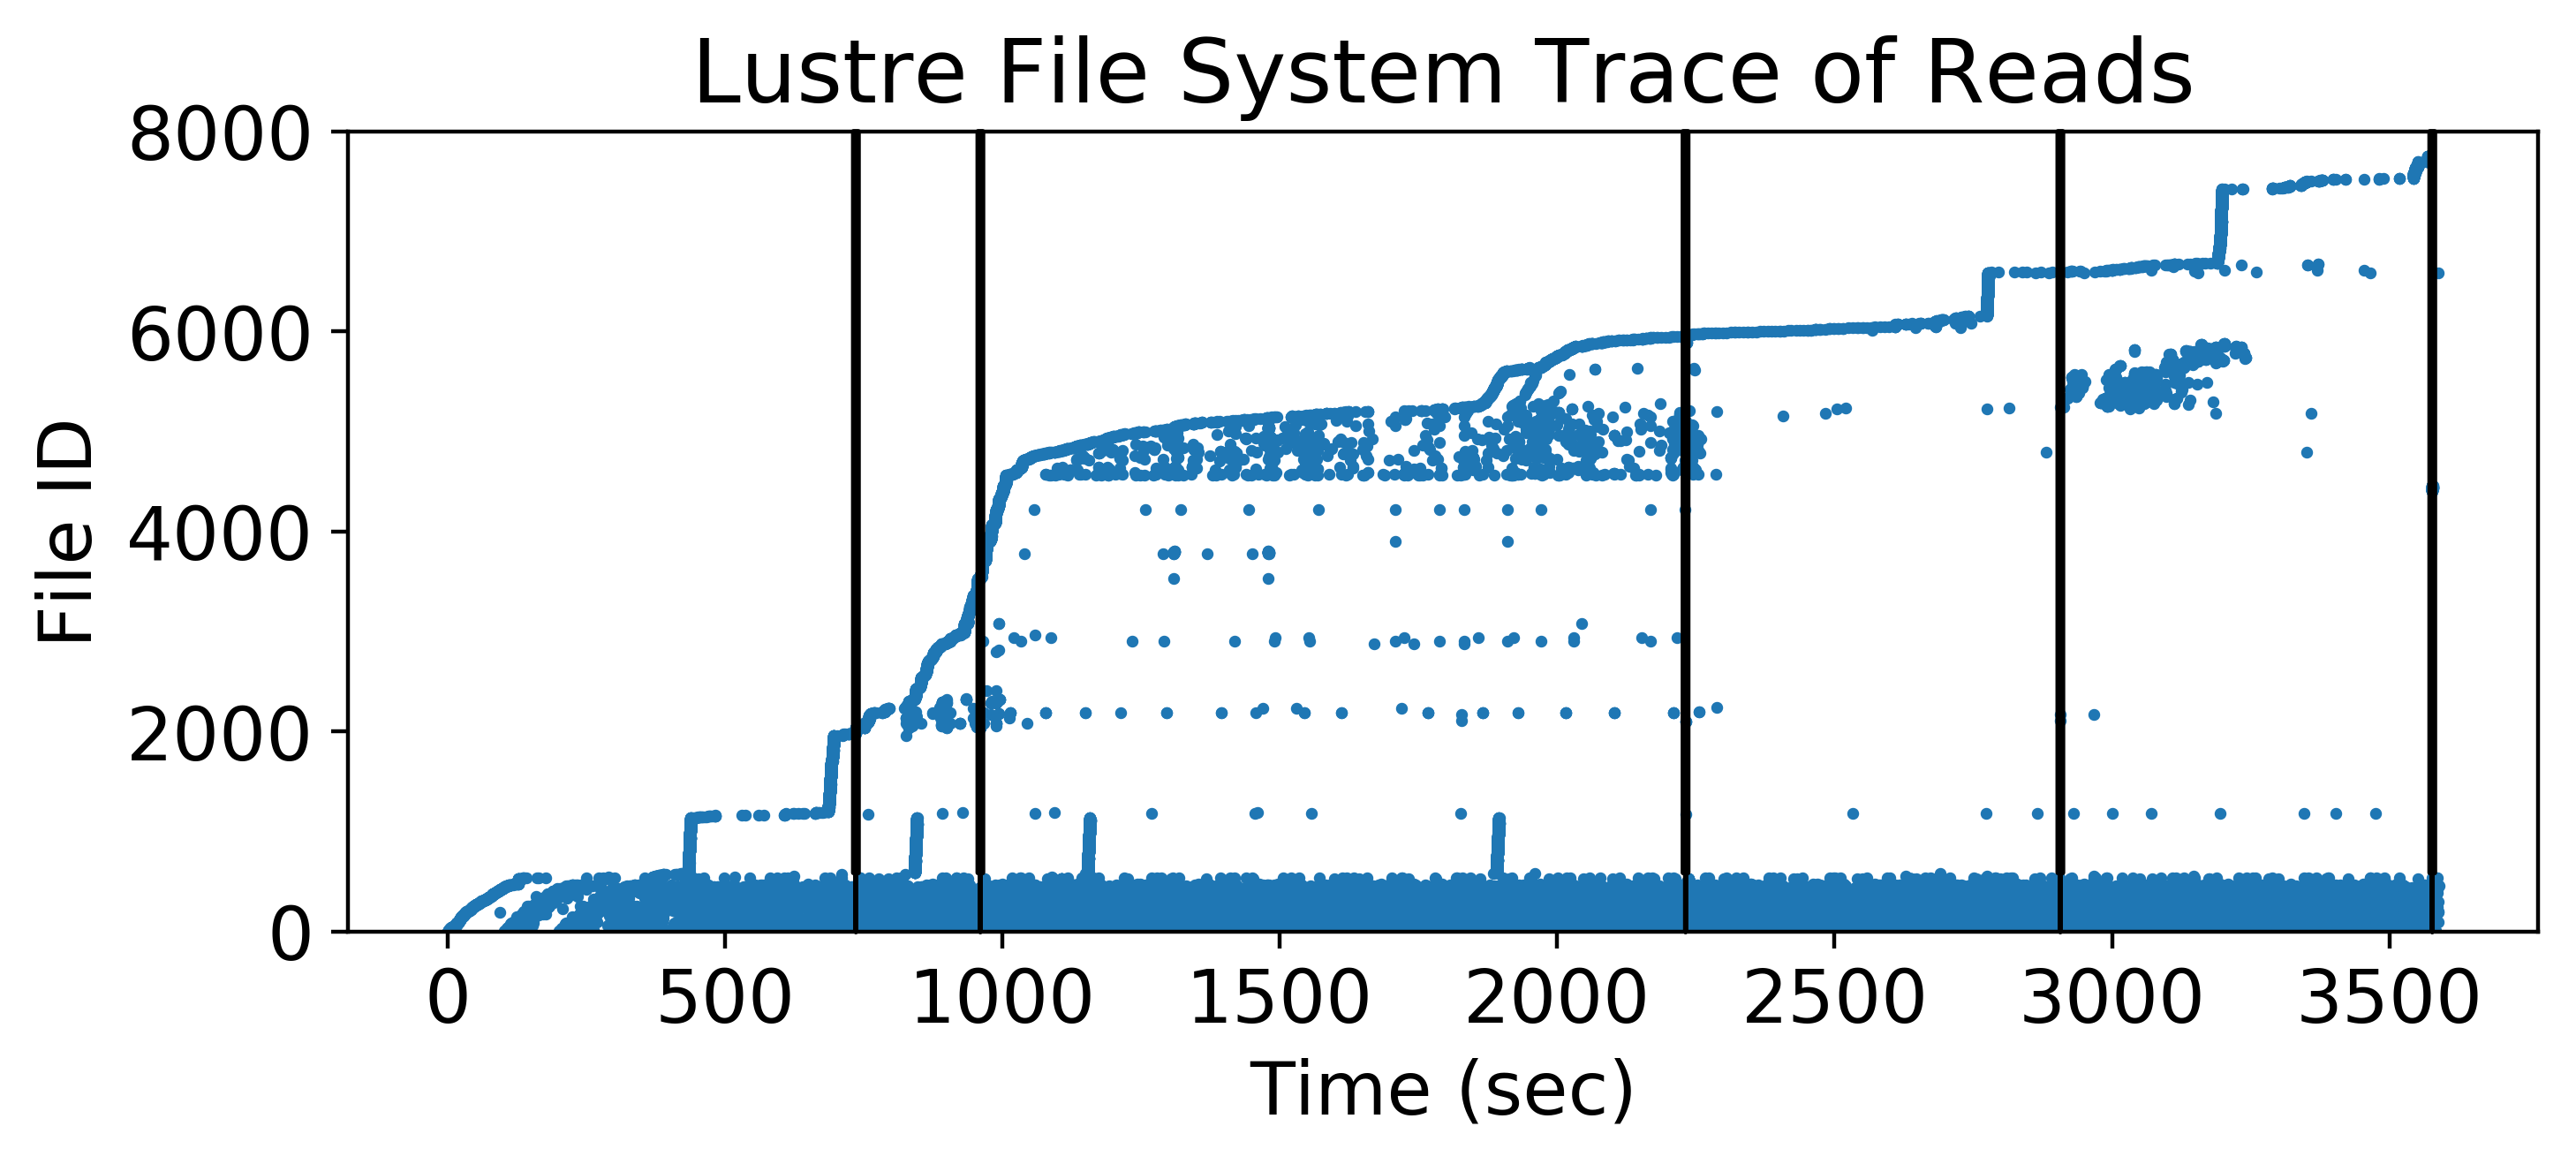
\includegraphics[width=0.9\textwidth]{./chapters/controlplane/parsplice/figures/trace-atime.png}\\
\caption{File system metadata reads for a Lustre trace collected at LANL. The
vertical lines are the access patterns detected by the ParSplice cache
management policy from Section~\S\ref{sec:dom-specific}. A file system that
load balances metadata across a cluster of servers could use the same pattern
detection to make migration decisions, such as avoiding migration when the
workload is accessing the same subset of keys or keeping groups of accesses
local to a server.  \label{fig:trace-atime}}
\end{figure}

%- how many inodes to keep in mds/client caches
%- affects LB; increases capacity of single MDS (reduces req/mem pressure)
%- affects LB; tells us which part of the cache to keep local

The cache management policies we developed earlier can be used by load
balancing policies to effectively spread load across a cluster. For example,
distributed file systems that load balance file system metadata across a
dedicated metadata cluster could use the caching policies to determine what
metadata to move and when to move it.  To demonstrate this idea, we analyze a
3-day Lustre file system metadata trace, collected at LANL.  The trace is
anonymized so all file names are replaced with a unique identifier and we do
not know which applications are running. We visualize a 1 hour window of the
trace in Figure~\ref{fig:trace-atime}, where the dots are the file system
metadata reads in a 1 hour window.  The \(x\) axis is time and the \(y\) axis
is the file ID, listed in the order that file IDs appear in the trace.  The
groups of accesses look similar to the ParSplice key accesses in
Figure~\ref{fig:keyspace-zoomed}. 

Although other access pattern detection algorithms are possible, we use the one
designed for cache management in Section~\S\ref{sec:regime-detection} with
slight modifications based on our knowledge of file systems\footnote{We
filtered out requests for key IDs less than 2000, as these are most likely path
traversal requests to higher parts of the namespace.}. The vertical lines in
Figure~\ref{fig:trace-atime} are the groups of accesses identified by the
algorithm; it successfully detects the largest group of key accesses that
starts at time 1000 seconds and ends at time 2200 seconds. File systems that
load balance file system metadata across a cluster would want to keep metadata
in that group of key accesses on the same server for locality and would want to
avoid migrating metadata to a different server until the group of key accesses
completes.

Before we showed how policies designed for load balancing heavily influence our
cache management in a different application and storage system. But in this
section we show how an {\it unmodified} cache management policy can be used in
a load balancing strategy.  This generalization may reduce the work that needs to
be done for load balancing as ideas may have already been explored in other
domains and could work ``out-of-the-box". 

%% burstiness of creates then compile
%Cache management can also increase the capacity of a single server, which
%affects how load should be distributed across a cluster.  For example, CephFS
%clients and servers maintain a consistent cache so that the client can do
%operations locally without contacting the metadata server.  But large caches
%use more memory, so having smart policies that detect key access patterns would
%greatly reduce memory footprints. For example, Figure~\ref{fig:compile-ops}
%shows the trace of metadata requests for compiling code in CephFS.  The \(y\)
%axis is  the number of file system metadata requests serviced by the metadata
%server when uncompressing (\texttt{untar}), compiling (\texttt{make}), and
%deleting (\texttt{rm}) the source code for the Linux kernel. If the system
%knows that the job phases would progress from many creates, to many lookups, to
%many deletes, then it could size its caches accordingly. For example, the file
%system could cache none of the metadata from the \texttt{untar} phase and run
%key access pattern detection during the \texttt{make} phase, resulting in the
%metadata server/clients only caching metadata that is repeatedly used. For the
%job in Figure~\ref{fig:compile-ops}, this would fill up the cache to only 20K
%inodes (the unit of metadata for file systems) instead of 60K, resulting in
%almost 40MB of memory savings (since an inode is about
%1KB\footnote{http://docs.ceph.com/docs/master/dev/mds\_internals/data-structures/})
%without sacrificing performance.
%
%%- strategy: cache all inodes on create
%\begin{figure}[t]
%\noindent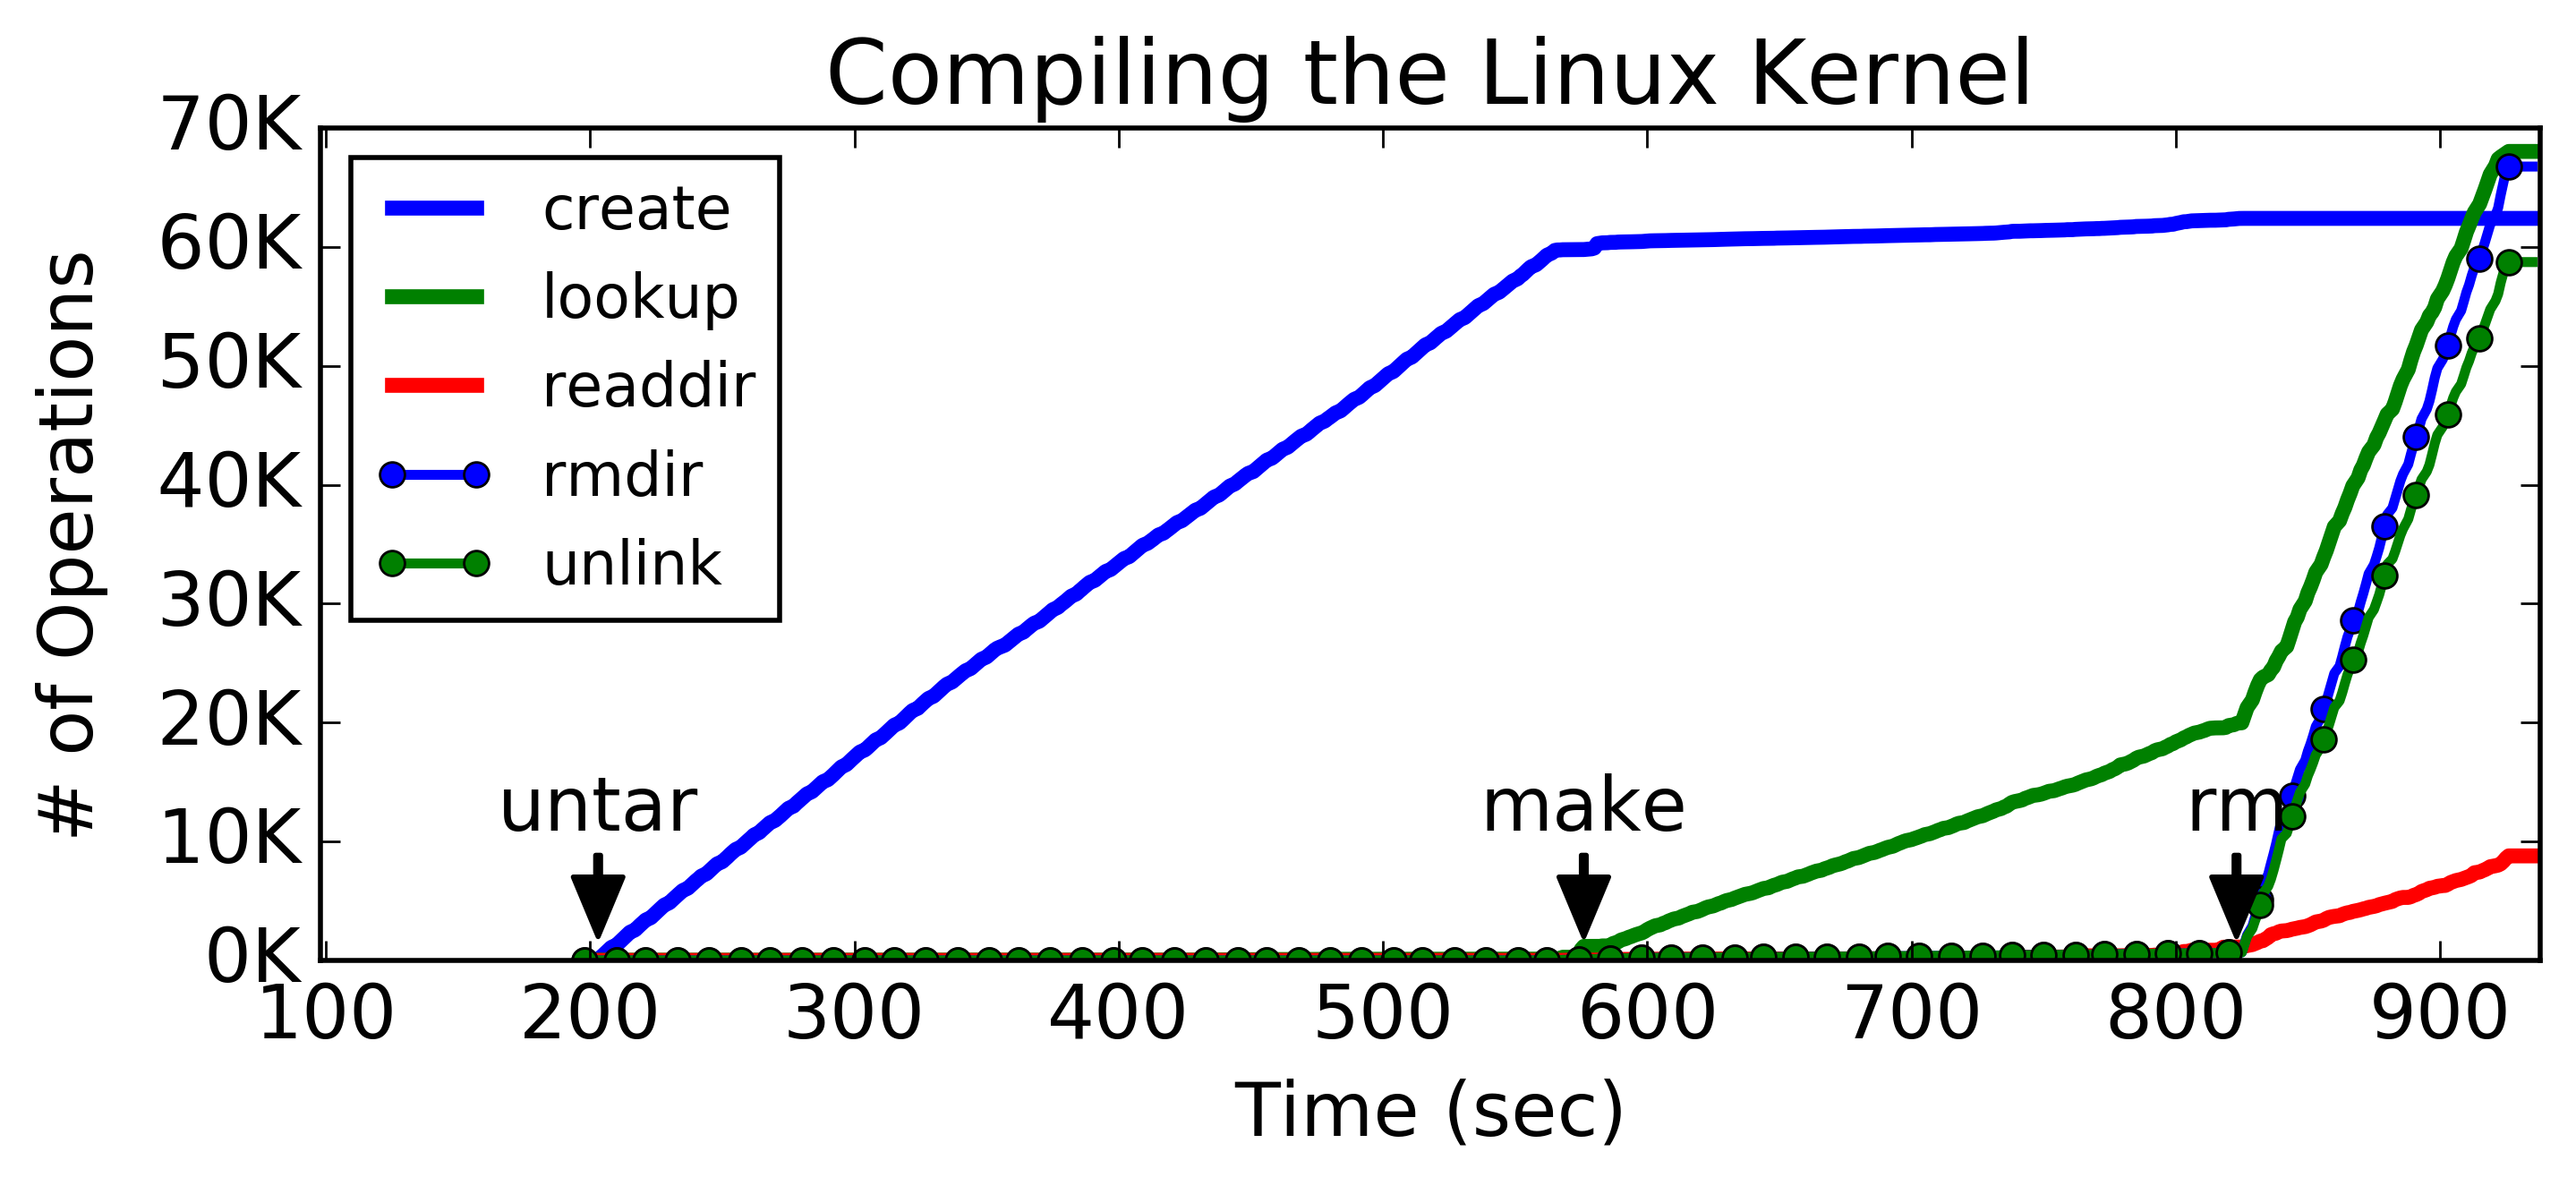
\includegraphics[width=0.5\textwidth]{./chapters/controlplane/parsplice/figures/compile-ops.png}\\
%\caption{File system metadata requests for a compile job show workload phases
%characterized by a dominant request type ({\it e.g.}, creates for ``untar").
%Using ParSplice cache management policies for these types of workloads would
%reduce memory pressure without sacrificing performance.
%\label{fig:compile-ops}}
%\end{figure}

\subsubsection{Other Use Cases}

% other use cases caches/tiers 
Storage systems have many other data management techniques that would benefit
from the caching policies developed in Sections~\S\ref{sec:arch-specific}
and~\S\ref{sec:dom-specific}. For example, Ceph administrators can use the
policies in ParSplice to automatically size and manage cache
tiers\footnote{http://docs.ceph.com/docs/master/rados/operations/cache-tiering/},
caching on object storage devices, or in the distributed block
devices\footnote{http://docs.ceph.com/docs/master/rbd/rbd-config-ref/}.
Integration with Mantle would be straightforward as it is merged into Ceph's
mainline\footnote{http://docs.ceph.com/docs/master/cephfs/mantle/} and the
three caching subsystems mentioned above already maintain key access traces. 

More generally, the similarities between load balancing and cache management
show how the ``when"/``where"/``how much" abstractions, data management
language, and policy engine may be widely applicable to other data management
techniques, such as:

\begin{itemize}

  \item QoS: when to move clients, where to move clients, how much of the
reservation to move. We could use Mantle to implement something like the
reservation algorithms based on utilization and period in
Fahrrad~\cite{povzner_horizon_2010} to achieve better guarantees without
sacrificing performance.

  \item Scheduling: when to yield computation cycles to another process, how
much of a resource to allocate. We could use Mantle to implement the
fairness/priority models used in the Mesos~\cite{hindman_mesos_2011} ``how
many" policies.

  \item Batching: how many operations to group together, when to send large
batches of updates. We could use Mantle to implement pathname leases from
IndexFS~\cite{ren:sc2014-indexfs} or the capabilities from
CephFS\footnote{http://docs.ceph.com/docs/master/cephfs/capabilities/}.

  \item Prefetching: how much to prefetch, how to select data.  We could use
Mantle to implement forward/backward/stride detection algorithms for
prefetching in RAID arrays or something more complicated, like the time series
algorithms for adaptive I/O prefetching from~\cite{tran:sc01-arima}.

\end{itemize}
